
The controller system’s architecture has been modelled such that the safety and liveness requirements are always met, by using the various sensors, actuators, and other components that are present in the system.

The main assumptions made here for simplicity are as follows. The robots perform the instructed actions without any error. The lamp performs the projecting process without malfunctioning. The other components may require the user to act upon them based on certain sensor data and the corresponding user inputs described as interactions in chapter~{\ref{chap:interact}}.

\begin{figure}[h]
\centering
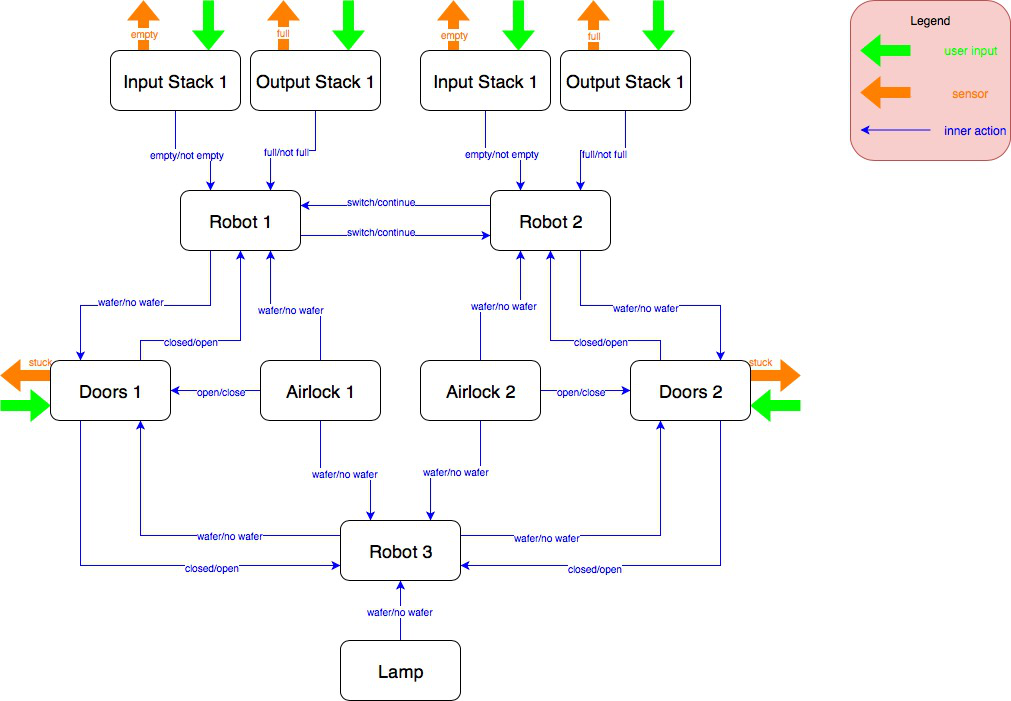
\includegraphics[width=150mm]{img/sv-project-arch.png}
\caption{System architecture diagram\label{fig:arch}}
\end{figure}

The architecture of the system is represented graphically using the Figure~{\ref{fig:arch}}. It consists of several components working in parallel to meet the requirements stated in chapter~{\ref{chap:reqs}}.

For the most part, the system is expected to function without the need for any user input, but certain cases have been identified in which "external interaction" is needed to meet the system’s liveness requirements. These are indicated by green arrows in the diagram. There are various controllers for the components, and communication between the controllers is represented using blue arrows. These interactions take place between the controllers continuously and ensure that the system runs automatically.

The controllers send the state of their associated components and poll for the states of other components as required, and make state transitions by performing the appropriate actions. The state transitions should not end up causing a deadlock within the overall system, at any cost. 

The system never reaches a state of “completion” since it is expected to run continuously till one of the conditions requiring an external interaction is met (see chapter~{\ref{chap:reqs}}). Theoretically, if the user continually replenishes the input stack with new wafers and clears the output stack at the same rate, and if the airlock doors do not malfunction, the system can run for an indefinite period of time.
